% Created by tikzDevice version 0.12.3.1 on 2021-06-13 15:08:26
% !TEX encoding = UTF-8 Unicode
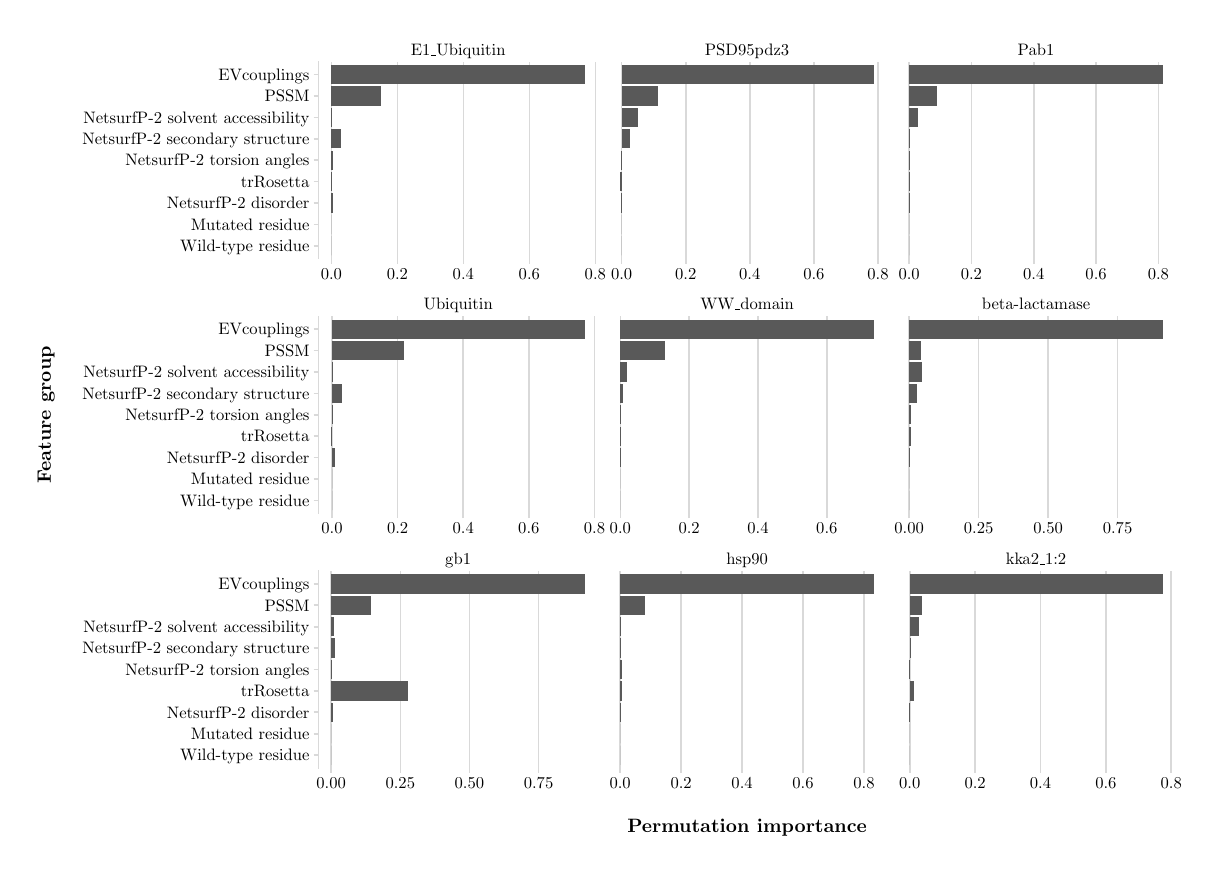
\begin{tikzpicture}[x=1pt,y=1pt]
\definecolor{fillColor}{RGB}{255,255,255}
\path[use as bounding box,fill=fillColor,fill opacity=0.00] (0,0) rectangle (418.34,295.82);
\begin{scope}
\path[clip] (105.09,212.35) rectangle (206.00,283.52);
\definecolor{drawColor}{gray}{0.85}

\path[draw=drawColor,line width= 0.6pt,line join=round] (109.74,212.35) --
	(109.74,283.52);

\path[draw=drawColor,line width= 0.6pt,line join=round] (133.59,212.35) --
	(133.59,283.52);

\path[draw=drawColor,line width= 0.6pt,line join=round] (157.43,212.35) --
	(157.43,283.52);

\path[draw=drawColor,line width= 0.6pt,line join=round] (181.28,212.35) --
	(181.28,283.52);

\path[draw=drawColor,line width= 0.6pt,line join=round] (205.13,212.35) --
	(205.13,283.52);
\definecolor{fillColor}{gray}{0.35}

\path[fill=fillColor] (109.68,236.72) rectangle (109.74,243.68);

\path[fill=fillColor] (109.74,267.66) rectangle (127.58,274.63);

\path[fill=fillColor] (109.74,259.93) rectangle (109.96,266.89);

\path[fill=fillColor] (109.74,252.19) rectangle (113.10,259.15);

\path[fill=fillColor] (109.74,228.98) rectangle (110.46,235.95);

\path[fill=fillColor] (109.74,244.46) rectangle (110.31,251.42);

\path[fill=fillColor] (109.74,275.40) rectangle (201.42,282.36);

\path[fill=fillColor] (109.74,213.51) rectangle (109.74,220.47);

\path[fill=fillColor] (109.74,221.25) rectangle (109.74,228.21);
\end{scope}
\begin{scope}
\path[clip] (105.09,120.33) rectangle (206.00,191.50);
\definecolor{drawColor}{gray}{0.85}

\path[draw=drawColor,line width= 0.6pt,line join=round] (109.98,120.33) --
	(109.98,191.50);

\path[draw=drawColor,line width= 0.6pt,line join=round] (133.69,120.33) --
	(133.69,191.50);

\path[draw=drawColor,line width= 0.6pt,line join=round] (157.39,120.33) --
	(157.39,191.50);

\path[draw=drawColor,line width= 0.6pt,line join=round] (181.10,120.33) --
	(181.10,191.50);

\path[draw=drawColor,line width= 0.6pt,line join=round] (204.81,120.33) --
	(204.81,191.50);
\definecolor{fillColor}{gray}{0.35}

\path[fill=fillColor] (109.68,144.70) rectangle (109.98,151.66);

\path[fill=fillColor] (109.98,175.64) rectangle (135.96,182.60);

\path[fill=fillColor] (109.98,167.90) rectangle (110.06,174.87);

\path[fill=fillColor] (109.98,160.17) rectangle (113.46,167.13);

\path[fill=fillColor] (109.98,136.96) rectangle (110.98,143.92);

\path[fill=fillColor] (109.98,152.43) rectangle (110.47,159.39);

\path[fill=fillColor] (109.98,183.38) rectangle (201.42,190.34);

\path[fill=fillColor] (109.98,121.49) rectangle (109.98,128.45);

\path[fill=fillColor] (109.98,129.22) rectangle (109.98,136.19);
\end{scope}
\begin{scope}
\path[clip] (105.09, 28.30) rectangle (206.00, 99.48);
\definecolor{drawColor}{gray}{0.85}

\path[draw=drawColor,line width= 0.6pt,line join=round] (109.68, 28.30) --
	(109.68, 99.48);

\path[draw=drawColor,line width= 0.6pt,line join=round] (134.66, 28.30) --
	(134.66, 99.48);

\path[draw=drawColor,line width= 0.6pt,line join=round] (159.63, 28.30) --
	(159.63, 99.48);

\path[draw=drawColor,line width= 0.6pt,line join=round] (184.61, 28.30) --
	(184.61, 99.48);
\definecolor{fillColor}{gray}{0.35}

\path[fill=fillColor] (109.68, 52.67) rectangle (137.25, 59.64);

\path[fill=fillColor] (109.68, 83.62) rectangle (124.11, 90.58);

\path[fill=fillColor] (109.68, 75.88) rectangle (110.53, 82.84);

\path[fill=fillColor] (109.68, 68.15) rectangle (110.88, 75.11);

\path[fill=fillColor] (109.68, 44.94) rectangle (110.23, 51.90);

\path[fill=fillColor] (109.68, 60.41) rectangle (110.06, 67.37);

\path[fill=fillColor] (109.68, 91.35) rectangle (201.42, 98.32);

\path[fill=fillColor] (109.68, 29.46) rectangle (109.68, 36.43);

\path[fill=fillColor] (109.68, 37.20) rectangle (109.68, 44.16);
\end{scope}
\begin{scope}
\path[clip] (209.50,212.35) rectangle (310.42,283.52);
\definecolor{drawColor}{gray}{0.85}

\path[draw=drawColor,line width= 0.6pt,line join=round] (214.62,212.35) --
	(214.62,283.52);

\path[draw=drawColor,line width= 0.6pt,line join=round] (237.78,212.35) --
	(237.78,283.52);

\path[draw=drawColor,line width= 0.6pt,line join=round] (260.94,212.35) --
	(260.94,283.52);

\path[draw=drawColor,line width= 0.6pt,line join=round] (284.10,212.35) --
	(284.10,283.52);

\path[draw=drawColor,line width= 0.6pt,line join=round] (307.26,212.35) --
	(307.26,283.52);
\definecolor{fillColor}{gray}{0.35}

\path[fill=fillColor] (214.09,236.72) rectangle (214.62,243.68);

\path[fill=fillColor] (214.62,267.66) rectangle (227.87,274.63);

\path[fill=fillColor] (214.62,259.93) rectangle (220.46,266.89);

\path[fill=fillColor] (214.62,252.19) rectangle (217.79,259.15);

\path[fill=fillColor] (214.48,228.98) rectangle (214.62,235.95);

\path[fill=fillColor] (214.47,244.46) rectangle (214.62,251.42);

\path[fill=fillColor] (214.62,275.40) rectangle (305.83,282.36);

\path[fill=fillColor] (214.62,213.51) rectangle (214.62,220.47);

\path[fill=fillColor] (214.62,221.25) rectangle (214.62,228.21);
\end{scope}
\begin{scope}
\path[clip] (209.50,120.33) rectangle (310.42,191.50);
\definecolor{drawColor}{gray}{0.85}

\path[draw=drawColor,line width= 0.6pt,line join=round] (214.16,120.33) --
	(214.16,191.50);

\path[draw=drawColor,line width= 0.6pt,line join=round] (239.03,120.33) --
	(239.03,191.50);

\path[draw=drawColor,line width= 0.6pt,line join=round] (263.90,120.33) --
	(263.90,191.50);

\path[draw=drawColor,line width= 0.6pt,line join=round] (288.77,120.33) --
	(288.77,191.50);
\definecolor{fillColor}{gray}{0.35}

\path[fill=fillColor] (214.16,144.70) rectangle (214.51,151.66);

\path[fill=fillColor] (214.16,175.64) rectangle (230.15,182.60);

\path[fill=fillColor] (214.16,167.90) rectangle (216.39,174.87);

\path[fill=fillColor] (214.16,160.17) rectangle (214.99,167.13);

\path[fill=fillColor] (214.09,136.96) rectangle (214.16,143.92);

\path[fill=fillColor] (214.16,152.43) rectangle (214.46,159.39);

\path[fill=fillColor] (214.16,183.38) rectangle (305.83,190.34);

\path[fill=fillColor] (214.16,121.49) rectangle (214.16,128.45);

\path[fill=fillColor] (214.16,129.22) rectangle (214.16,136.19);
\end{scope}
\begin{scope}
\path[clip] (209.50, 28.30) rectangle (310.42, 99.48);
\definecolor{drawColor}{gray}{0.85}

\path[draw=drawColor,line width= 0.6pt,line join=round] (214.09, 28.30) --
	(214.09, 99.48);

\path[draw=drawColor,line width= 0.6pt,line join=round] (236.12, 28.30) --
	(236.12, 99.48);

\path[draw=drawColor,line width= 0.6pt,line join=round] (258.15, 28.30) --
	(258.15, 99.48);

\path[draw=drawColor,line width= 0.6pt,line join=round] (280.17, 28.30) --
	(280.17, 99.48);

\path[draw=drawColor,line width= 0.6pt,line join=round] (302.20, 28.30) --
	(302.20, 99.48);
\definecolor{fillColor}{gray}{0.35}

\path[fill=fillColor] (214.09, 52.67) rectangle (214.65, 59.64);

\path[fill=fillColor] (214.09, 83.62) rectangle (223.23, 90.58);

\path[fill=fillColor] (214.09, 75.88) rectangle (214.26, 82.84);

\path[fill=fillColor] (214.09, 68.15) rectangle (214.29, 75.11);

\path[fill=fillColor] (214.09, 44.94) rectangle (214.34, 51.90);

\path[fill=fillColor] (214.09, 60.41) rectangle (214.83, 67.37);

\path[fill=fillColor] (214.09, 91.35) rectangle (305.83, 98.32);

\path[fill=fillColor] (214.09, 29.46) rectangle (214.09, 36.43);

\path[fill=fillColor] (214.09, 37.20) rectangle (214.09, 44.16);
\end{scope}
\begin{scope}
\path[clip] (313.92,212.35) rectangle (414.84,283.52);
\definecolor{drawColor}{gray}{0.85}

\path[draw=drawColor,line width= 0.6pt,line join=round] (318.51,212.35) --
	(318.51,283.52);

\path[draw=drawColor,line width= 0.6pt,line join=round] (341.03,212.35) --
	(341.03,283.52);

\path[draw=drawColor,line width= 0.6pt,line join=round] (363.55,212.35) --
	(363.55,283.52);

\path[draw=drawColor,line width= 0.6pt,line join=round] (386.07,212.35) --
	(386.07,283.52);

\path[draw=drawColor,line width= 0.6pt,line join=round] (408.59,212.35) --
	(408.59,283.52);
\definecolor{fillColor}{gray}{0.35}

\path[fill=fillColor] (318.51,236.72) rectangle (318.54,243.68);

\path[fill=fillColor] (318.51,267.66) rectangle (328.62,274.63);

\path[fill=fillColor] (318.51,259.93) rectangle (321.78,266.89);

\path[fill=fillColor] (318.51,252.19) rectangle (318.76,259.15);

\path[fill=fillColor] (318.51,228.98) rectangle (318.70,235.95);

\path[fill=fillColor] (318.51,244.46) rectangle (318.96,251.42);

\path[fill=fillColor] (318.51,275.40) rectangle (410.25,282.36);

\path[fill=fillColor] (318.51,213.51) rectangle (318.51,220.47);

\path[fill=fillColor] (318.51,221.25) rectangle (318.51,228.21);
\end{scope}
\begin{scope}
\path[clip] (313.92,120.33) rectangle (414.84,191.50);
\definecolor{drawColor}{gray}{0.85}

\path[draw=drawColor,line width= 0.6pt,line join=round] (318.51,120.33) --
	(318.51,191.50);

\path[draw=drawColor,line width= 0.6pt,line join=round] (343.62,120.33) --
	(343.62,191.50);

\path[draw=drawColor,line width= 0.6pt,line join=round] (368.73,120.33) --
	(368.73,191.50);

\path[draw=drawColor,line width= 0.6pt,line join=round] (393.84,120.33) --
	(393.84,191.50);
\definecolor{fillColor}{gray}{0.35}

\path[fill=fillColor] (318.51,144.70) rectangle (319.21,151.66);

\path[fill=fillColor] (318.51,175.64) rectangle (322.90,182.60);

\path[fill=fillColor] (318.51,167.90) rectangle (322.99,174.87);

\path[fill=fillColor] (318.51,160.17) rectangle (321.20,167.13);

\path[fill=fillColor] (318.51,136.96) rectangle (318.72,143.92);

\path[fill=fillColor] (318.51,152.43) rectangle (319.13,159.39);

\path[fill=fillColor] (318.51,183.38) rectangle (410.25,190.34);

\path[fill=fillColor] (318.51,121.49) rectangle (318.51,128.45);

\path[fill=fillColor] (318.51,129.22) rectangle (318.51,136.19);
\end{scope}
\begin{scope}
\path[clip] (313.92, 28.30) rectangle (414.84, 99.48);
\definecolor{drawColor}{gray}{0.85}

\path[draw=drawColor,line width= 0.6pt,line join=round] (318.75, 28.30) --
	(318.75, 99.48);

\path[draw=drawColor,line width= 0.6pt,line join=round] (342.37, 28.30) --
	(342.37, 99.48);

\path[draw=drawColor,line width= 0.6pt,line join=round] (365.99, 28.30) --
	(365.99, 99.48);

\path[draw=drawColor,line width= 0.6pt,line join=round] (389.61, 28.30) --
	(389.61, 99.48);

\path[draw=drawColor,line width= 0.6pt,line join=round] (413.22, 28.30) --
	(413.22, 99.48);
\definecolor{fillColor}{gray}{0.35}

\path[fill=fillColor] (318.75, 52.67) rectangle (320.40, 59.64);

\path[fill=fillColor] (318.75, 83.62) rectangle (323.34, 90.58);

\path[fill=fillColor] (318.75, 75.88) rectangle (322.03, 82.84);

\path[fill=fillColor] (318.75, 68.15) rectangle (318.81, 75.11);

\path[fill=fillColor] (318.59, 44.94) rectangle (318.75, 51.90);

\path[fill=fillColor] (318.51, 60.41) rectangle (318.75, 67.37);

\path[fill=fillColor] (318.75, 91.35) rectangle (410.25, 98.32);

\path[fill=fillColor] (318.75, 29.46) rectangle (318.75, 36.43);

\path[fill=fillColor] (318.75, 37.20) rectangle (318.75, 44.16);
\end{scope}
\begin{scope}
\path[clip] (105.09, 99.48) rectangle (206.00,108.28);
\definecolor{drawColor}{RGB}{0,0,0}

\node[text=drawColor,anchor=base,inner sep=0pt, outer sep=0pt, scale=  0.60] at (155.55,101.81) {gb1};
\end{scope}
\begin{scope}
\path[clip] (209.50, 99.48) rectangle (310.42,108.28);
\definecolor{drawColor}{RGB}{0,0,0}

\node[text=drawColor,anchor=base,inner sep=0pt, outer sep=0pt, scale=  0.60] at (259.96,101.81) {hsp90};
\end{scope}
\begin{scope}
\path[clip] (313.92, 99.48) rectangle (414.84,108.28);
\definecolor{drawColor}{RGB}{0,0,0}

\node[text=drawColor,anchor=base,inner sep=0pt, outer sep=0pt, scale=  0.60] at (364.38,101.81) {kka2\_1:2};
\end{scope}
\begin{scope}
\path[clip] (105.09,191.50) rectangle (206.00,200.30);
\definecolor{drawColor}{RGB}{0,0,0}

\node[text=drawColor,anchor=base,inner sep=0pt, outer sep=0pt, scale=  0.60] at (155.55,193.83) {Ubiquitin};
\end{scope}
\begin{scope}
\path[clip] (209.50,191.50) rectangle (310.42,200.30);
\definecolor{drawColor}{RGB}{0,0,0}

\node[text=drawColor,anchor=base,inner sep=0pt, outer sep=0pt, scale=  0.60] at (259.96,193.83) {WW\_domain};
\end{scope}
\begin{scope}
\path[clip] (313.92,191.50) rectangle (414.84,200.30);
\definecolor{drawColor}{RGB}{0,0,0}

\node[text=drawColor,anchor=base,inner sep=0pt, outer sep=0pt, scale=  0.60] at (364.38,193.83) {beta-lactamase};
\end{scope}
\begin{scope}
\path[clip] (105.09,283.52) rectangle (206.00,292.32);
\definecolor{drawColor}{RGB}{0,0,0}

\node[text=drawColor,anchor=base,inner sep=0pt, outer sep=0pt, scale=  0.60] at (155.55,285.86) {E1\_Ubiquitin};
\end{scope}
\begin{scope}
\path[clip] (209.50,283.52) rectangle (310.42,292.32);
\definecolor{drawColor}{RGB}{0,0,0}

\node[text=drawColor,anchor=base,inner sep=0pt, outer sep=0pt, scale=  0.60] at (259.96,285.86) {PSD95pdz3};
\end{scope}
\begin{scope}
\path[clip] (313.92,283.52) rectangle (414.84,292.32);
\definecolor{drawColor}{RGB}{0,0,0}

\node[text=drawColor,anchor=base,inner sep=0pt, outer sep=0pt, scale=  0.60] at (364.38,285.86) {Pab1};
\end{scope}
\begin{scope}
\path[clip] (  0.00,  0.00) rectangle (418.34,295.82);
\definecolor{drawColor}{gray}{0.85}

\path[draw=drawColor,line width= 0.6pt,line join=round] (109.68, 26.55) --
	(109.68, 28.30);

\path[draw=drawColor,line width= 0.6pt,line join=round] (134.66, 26.55) --
	(134.66, 28.30);

\path[draw=drawColor,line width= 0.6pt,line join=round] (159.63, 26.55) --
	(159.63, 28.30);

\path[draw=drawColor,line width= 0.6pt,line join=round] (184.61, 26.55) --
	(184.61, 28.30);
\end{scope}
\begin{scope}
\path[clip] (  0.00,  0.00) rectangle (418.34,295.82);
\definecolor{drawColor}{RGB}{0,0,0}

\node[text=drawColor,anchor=base,inner sep=0pt, outer sep=0pt, scale=  0.60] at (109.68, 20.92) {0.00};

\node[text=drawColor,anchor=base,inner sep=0pt, outer sep=0pt, scale=  0.60] at (134.66, 20.92) {0.25};

\node[text=drawColor,anchor=base,inner sep=0pt, outer sep=0pt, scale=  0.60] at (159.63, 20.92) {0.50};

\node[text=drawColor,anchor=base,inner sep=0pt, outer sep=0pt, scale=  0.60] at (184.61, 20.92) {0.75};
\end{scope}
\begin{scope}
\path[clip] (  0.00,  0.00) rectangle (418.34,295.82);
\definecolor{drawColor}{gray}{0.85}

\path[draw=drawColor,line width= 0.6pt,line join=round] (214.09, 26.55) --
	(214.09, 28.30);

\path[draw=drawColor,line width= 0.6pt,line join=round] (236.12, 26.55) --
	(236.12, 28.30);

\path[draw=drawColor,line width= 0.6pt,line join=round] (258.15, 26.55) --
	(258.15, 28.30);

\path[draw=drawColor,line width= 0.6pt,line join=round] (280.17, 26.55) --
	(280.17, 28.30);

\path[draw=drawColor,line width= 0.6pt,line join=round] (302.20, 26.55) --
	(302.20, 28.30);
\end{scope}
\begin{scope}
\path[clip] (  0.00,  0.00) rectangle (418.34,295.82);
\definecolor{drawColor}{RGB}{0,0,0}

\node[text=drawColor,anchor=base,inner sep=0pt, outer sep=0pt, scale=  0.60] at (214.09, 20.92) {0.0};

\node[text=drawColor,anchor=base,inner sep=0pt, outer sep=0pt, scale=  0.60] at (236.12, 20.92) {0.2};

\node[text=drawColor,anchor=base,inner sep=0pt, outer sep=0pt, scale=  0.60] at (258.15, 20.92) {0.4};

\node[text=drawColor,anchor=base,inner sep=0pt, outer sep=0pt, scale=  0.60] at (280.17, 20.92) {0.6};

\node[text=drawColor,anchor=base,inner sep=0pt, outer sep=0pt, scale=  0.60] at (302.20, 20.92) {0.8};
\end{scope}
\begin{scope}
\path[clip] (  0.00,  0.00) rectangle (418.34,295.82);
\definecolor{drawColor}{gray}{0.85}

\path[draw=drawColor,line width= 0.6pt,line join=round] (318.75, 26.55) --
	(318.75, 28.30);

\path[draw=drawColor,line width= 0.6pt,line join=round] (342.37, 26.55) --
	(342.37, 28.30);

\path[draw=drawColor,line width= 0.6pt,line join=round] (365.99, 26.55) --
	(365.99, 28.30);

\path[draw=drawColor,line width= 0.6pt,line join=round] (389.61, 26.55) --
	(389.61, 28.30);

\path[draw=drawColor,line width= 0.6pt,line join=round] (413.22, 26.55) --
	(413.22, 28.30);
\end{scope}
\begin{scope}
\path[clip] (  0.00,  0.00) rectangle (418.34,295.82);
\definecolor{drawColor}{RGB}{0,0,0}

\node[text=drawColor,anchor=base,inner sep=0pt, outer sep=0pt, scale=  0.60] at (318.75, 20.92) {0.0};

\node[text=drawColor,anchor=base,inner sep=0pt, outer sep=0pt, scale=  0.60] at (342.37, 20.92) {0.2};

\node[text=drawColor,anchor=base,inner sep=0pt, outer sep=0pt, scale=  0.60] at (365.99, 20.92) {0.4};

\node[text=drawColor,anchor=base,inner sep=0pt, outer sep=0pt, scale=  0.60] at (389.61, 20.92) {0.6};

\node[text=drawColor,anchor=base,inner sep=0pt, outer sep=0pt, scale=  0.60] at (413.22, 20.92) {0.8};
\end{scope}
\begin{scope}
\path[clip] (  0.00,  0.00) rectangle (418.34,295.82);
\definecolor{drawColor}{gray}{0.85}

\path[draw=drawColor,line width= 0.6pt,line join=round] (109.98,118.58) --
	(109.98,120.33);

\path[draw=drawColor,line width= 0.6pt,line join=round] (133.69,118.58) --
	(133.69,120.33);

\path[draw=drawColor,line width= 0.6pt,line join=round] (157.39,118.58) --
	(157.39,120.33);

\path[draw=drawColor,line width= 0.6pt,line join=round] (181.10,118.58) --
	(181.10,120.33);

\path[draw=drawColor,line width= 0.6pt,line join=round] (204.81,118.58) --
	(204.81,120.33);
\end{scope}
\begin{scope}
\path[clip] (  0.00,  0.00) rectangle (418.34,295.82);
\definecolor{drawColor}{RGB}{0,0,0}

\node[text=drawColor,anchor=base,inner sep=0pt, outer sep=0pt, scale=  0.60] at (109.98,112.94) {0.0};

\node[text=drawColor,anchor=base,inner sep=0pt, outer sep=0pt, scale=  0.60] at (133.69,112.94) {0.2};

\node[text=drawColor,anchor=base,inner sep=0pt, outer sep=0pt, scale=  0.60] at (157.39,112.94) {0.4};

\node[text=drawColor,anchor=base,inner sep=0pt, outer sep=0pt, scale=  0.60] at (181.10,112.94) {0.6};

\node[text=drawColor,anchor=base,inner sep=0pt, outer sep=0pt, scale=  0.60] at (204.81,112.94) {0.8};
\end{scope}
\begin{scope}
\path[clip] (  0.00,  0.00) rectangle (418.34,295.82);
\definecolor{drawColor}{gray}{0.85}

\path[draw=drawColor,line width= 0.6pt,line join=round] (214.16,118.58) --
	(214.16,120.33);

\path[draw=drawColor,line width= 0.6pt,line join=round] (239.03,118.58) --
	(239.03,120.33);

\path[draw=drawColor,line width= 0.6pt,line join=round] (263.90,118.58) --
	(263.90,120.33);

\path[draw=drawColor,line width= 0.6pt,line join=round] (288.77,118.58) --
	(288.77,120.33);
\end{scope}
\begin{scope}
\path[clip] (  0.00,  0.00) rectangle (418.34,295.82);
\definecolor{drawColor}{RGB}{0,0,0}

\node[text=drawColor,anchor=base,inner sep=0pt, outer sep=0pt, scale=  0.60] at (214.16,112.94) {0.0};

\node[text=drawColor,anchor=base,inner sep=0pt, outer sep=0pt, scale=  0.60] at (239.03,112.94) {0.2};

\node[text=drawColor,anchor=base,inner sep=0pt, outer sep=0pt, scale=  0.60] at (263.90,112.94) {0.4};

\node[text=drawColor,anchor=base,inner sep=0pt, outer sep=0pt, scale=  0.60] at (288.77,112.94) {0.6};
\end{scope}
\begin{scope}
\path[clip] (  0.00,  0.00) rectangle (418.34,295.82);
\definecolor{drawColor}{gray}{0.85}

\path[draw=drawColor,line width= 0.6pt,line join=round] (318.51,118.58) --
	(318.51,120.33);

\path[draw=drawColor,line width= 0.6pt,line join=round] (343.62,118.58) --
	(343.62,120.33);

\path[draw=drawColor,line width= 0.6pt,line join=round] (368.73,118.58) --
	(368.73,120.33);

\path[draw=drawColor,line width= 0.6pt,line join=round] (393.84,118.58) --
	(393.84,120.33);
\end{scope}
\begin{scope}
\path[clip] (  0.00,  0.00) rectangle (418.34,295.82);
\definecolor{drawColor}{RGB}{0,0,0}

\node[text=drawColor,anchor=base,inner sep=0pt, outer sep=0pt, scale=  0.60] at (318.51,112.94) {0.00};

\node[text=drawColor,anchor=base,inner sep=0pt, outer sep=0pt, scale=  0.60] at (343.62,112.94) {0.25};

\node[text=drawColor,anchor=base,inner sep=0pt, outer sep=0pt, scale=  0.60] at (368.73,112.94) {0.50};

\node[text=drawColor,anchor=base,inner sep=0pt, outer sep=0pt, scale=  0.60] at (393.84,112.94) {0.75};
\end{scope}
\begin{scope}
\path[clip] (  0.00,  0.00) rectangle (418.34,295.82);
\definecolor{drawColor}{gray}{0.85}

\path[draw=drawColor,line width= 0.6pt,line join=round] (109.74,210.60) --
	(109.74,212.35);

\path[draw=drawColor,line width= 0.6pt,line join=round] (133.59,210.60) --
	(133.59,212.35);

\path[draw=drawColor,line width= 0.6pt,line join=round] (157.43,210.60) --
	(157.43,212.35);

\path[draw=drawColor,line width= 0.6pt,line join=round] (181.28,210.60) --
	(181.28,212.35);

\path[draw=drawColor,line width= 0.6pt,line join=round] (205.13,210.60) --
	(205.13,212.35);
\end{scope}
\begin{scope}
\path[clip] (  0.00,  0.00) rectangle (418.34,295.82);
\definecolor{drawColor}{RGB}{0,0,0}

\node[text=drawColor,anchor=base,inner sep=0pt, outer sep=0pt, scale=  0.60] at (109.74,204.97) {0.0};

\node[text=drawColor,anchor=base,inner sep=0pt, outer sep=0pt, scale=  0.60] at (133.59,204.97) {0.2};

\node[text=drawColor,anchor=base,inner sep=0pt, outer sep=0pt, scale=  0.60] at (157.43,204.97) {0.4};

\node[text=drawColor,anchor=base,inner sep=0pt, outer sep=0pt, scale=  0.60] at (181.28,204.97) {0.6};

\node[text=drawColor,anchor=base,inner sep=0pt, outer sep=0pt, scale=  0.60] at (205.13,204.97) {0.8};
\end{scope}
\begin{scope}
\path[clip] (  0.00,  0.00) rectangle (418.34,295.82);
\definecolor{drawColor}{gray}{0.85}

\path[draw=drawColor,line width= 0.6pt,line join=round] (214.62,210.60) --
	(214.62,212.35);

\path[draw=drawColor,line width= 0.6pt,line join=round] (237.78,210.60) --
	(237.78,212.35);

\path[draw=drawColor,line width= 0.6pt,line join=round] (260.94,210.60) --
	(260.94,212.35);

\path[draw=drawColor,line width= 0.6pt,line join=round] (284.10,210.60) --
	(284.10,212.35);

\path[draw=drawColor,line width= 0.6pt,line join=round] (307.26,210.60) --
	(307.26,212.35);
\end{scope}
\begin{scope}
\path[clip] (  0.00,  0.00) rectangle (418.34,295.82);
\definecolor{drawColor}{RGB}{0,0,0}

\node[text=drawColor,anchor=base,inner sep=0pt, outer sep=0pt, scale=  0.60] at (214.62,204.97) {0.0};

\node[text=drawColor,anchor=base,inner sep=0pt, outer sep=0pt, scale=  0.60] at (237.78,204.97) {0.2};

\node[text=drawColor,anchor=base,inner sep=0pt, outer sep=0pt, scale=  0.60] at (260.94,204.97) {0.4};

\node[text=drawColor,anchor=base,inner sep=0pt, outer sep=0pt, scale=  0.60] at (284.10,204.97) {0.6};

\node[text=drawColor,anchor=base,inner sep=0pt, outer sep=0pt, scale=  0.60] at (307.26,204.97) {0.8};
\end{scope}
\begin{scope}
\path[clip] (  0.00,  0.00) rectangle (418.34,295.82);
\definecolor{drawColor}{gray}{0.85}

\path[draw=drawColor,line width= 0.6pt,line join=round] (318.51,210.60) --
	(318.51,212.35);

\path[draw=drawColor,line width= 0.6pt,line join=round] (341.03,210.60) --
	(341.03,212.35);

\path[draw=drawColor,line width= 0.6pt,line join=round] (363.55,210.60) --
	(363.55,212.35);

\path[draw=drawColor,line width= 0.6pt,line join=round] (386.07,210.60) --
	(386.07,212.35);

\path[draw=drawColor,line width= 0.6pt,line join=round] (408.59,210.60) --
	(408.59,212.35);
\end{scope}
\begin{scope}
\path[clip] (  0.00,  0.00) rectangle (418.34,295.82);
\definecolor{drawColor}{RGB}{0,0,0}

\node[text=drawColor,anchor=base,inner sep=0pt, outer sep=0pt, scale=  0.60] at (318.51,204.97) {0.0};

\node[text=drawColor,anchor=base,inner sep=0pt, outer sep=0pt, scale=  0.60] at (341.03,204.97) {0.2};

\node[text=drawColor,anchor=base,inner sep=0pt, outer sep=0pt, scale=  0.60] at (363.55,204.97) {0.4};

\node[text=drawColor,anchor=base,inner sep=0pt, outer sep=0pt, scale=  0.60] at (386.07,204.97) {0.6};

\node[text=drawColor,anchor=base,inner sep=0pt, outer sep=0pt, scale=  0.60] at (408.59,204.97) {0.8};
\end{scope}
\begin{scope}
\path[clip] (  0.00,  0.00) rectangle (418.34,295.82);
\definecolor{drawColor}{gray}{0.85}

\path[draw=drawColor,line width= 0.6pt,line join=round,line cap=rect] (105.09,212.35) --
	(105.09,283.52);
\end{scope}
\begin{scope}
\path[clip] (  0.00,  0.00) rectangle (418.34,295.82);
\definecolor{drawColor}{RGB}{0,0,0}

\node[text=drawColor,anchor=base east,inner sep=0pt, outer sep=0pt, scale=  0.60] at (101.84,214.92) {Wild-type residue};

\node[text=drawColor,anchor=base east,inner sep=0pt, outer sep=0pt, scale=  0.60] at (101.84,222.66) {Mutated residue};

\node[text=drawColor,anchor=base east,inner sep=0pt, outer sep=0pt, scale=  0.60] at (101.84,230.40) {NetsurfP-2 disorder};

\node[text=drawColor,anchor=base east,inner sep=0pt, outer sep=0pt, scale=  0.60] at (101.84,238.13) {trRosetta};

\node[text=drawColor,anchor=base east,inner sep=0pt, outer sep=0pt, scale=  0.60] at (101.84,245.87) {NetsurfP-2 torsion angles};

\node[text=drawColor,anchor=base east,inner sep=0pt, outer sep=0pt, scale=  0.60] at (101.84,253.61) {NetsurfP-2 secondary structure};

\node[text=drawColor,anchor=base east,inner sep=0pt, outer sep=0pt, scale=  0.60] at (101.84,261.34) {NetsurfP-2 solvent accessibility};

\node[text=drawColor,anchor=base east,inner sep=0pt, outer sep=0pt, scale=  0.60] at (101.84,269.08) {PSSM};

\node[text=drawColor,anchor=base east,inner sep=0pt, outer sep=0pt, scale=  0.60] at (101.84,276.81) {EVcouplings};
\end{scope}
\begin{scope}
\path[clip] (  0.00,  0.00) rectangle (418.34,295.82);
\definecolor{drawColor}{gray}{0.85}

\path[draw=drawColor,line width= 0.6pt,line join=round] (103.34,216.99) --
	(105.09,216.99);

\path[draw=drawColor,line width= 0.6pt,line join=round] (103.34,224.73) --
	(105.09,224.73);

\path[draw=drawColor,line width= 0.6pt,line join=round] (103.34,232.46) --
	(105.09,232.46);

\path[draw=drawColor,line width= 0.6pt,line join=round] (103.34,240.20) --
	(105.09,240.20);

\path[draw=drawColor,line width= 0.6pt,line join=round] (103.34,247.94) --
	(105.09,247.94);

\path[draw=drawColor,line width= 0.6pt,line join=round] (103.34,255.67) --
	(105.09,255.67);

\path[draw=drawColor,line width= 0.6pt,line join=round] (103.34,263.41) --
	(105.09,263.41);

\path[draw=drawColor,line width= 0.6pt,line join=round] (103.34,271.14) --
	(105.09,271.14);

\path[draw=drawColor,line width= 0.6pt,line join=round] (103.34,278.88) --
	(105.09,278.88);
\end{scope}
\begin{scope}
\path[clip] (  0.00,  0.00) rectangle (418.34,295.82);
\definecolor{drawColor}{gray}{0.85}

\path[draw=drawColor,line width= 0.6pt,line join=round,line cap=rect] (105.09,120.33) --
	(105.09,191.50);
\end{scope}
\begin{scope}
\path[clip] (  0.00,  0.00) rectangle (418.34,295.82);
\definecolor{drawColor}{RGB}{0,0,0}

\node[text=drawColor,anchor=base east,inner sep=0pt, outer sep=0pt, scale=  0.60] at (101.84,122.90) {Wild-type residue};

\node[text=drawColor,anchor=base east,inner sep=0pt, outer sep=0pt, scale=  0.60] at (101.84,130.64) {Mutated residue};

\node[text=drawColor,anchor=base east,inner sep=0pt, outer sep=0pt, scale=  0.60] at (101.84,138.37) {NetsurfP-2 disorder};

\node[text=drawColor,anchor=base east,inner sep=0pt, outer sep=0pt, scale=  0.60] at (101.84,146.11) {trRosetta};

\node[text=drawColor,anchor=base east,inner sep=0pt, outer sep=0pt, scale=  0.60] at (101.84,153.85) {NetsurfP-2 torsion angles};

\node[text=drawColor,anchor=base east,inner sep=0pt, outer sep=0pt, scale=  0.60] at (101.84,161.58) {NetsurfP-2 secondary structure};

\node[text=drawColor,anchor=base east,inner sep=0pt, outer sep=0pt, scale=  0.60] at (101.84,169.32) {NetsurfP-2 solvent accessibility};

\node[text=drawColor,anchor=base east,inner sep=0pt, outer sep=0pt, scale=  0.60] at (101.84,177.06) {PSSM};

\node[text=drawColor,anchor=base east,inner sep=0pt, outer sep=0pt, scale=  0.60] at (101.84,184.79) {EVcouplings};
\end{scope}
\begin{scope}
\path[clip] (  0.00,  0.00) rectangle (418.34,295.82);
\definecolor{drawColor}{gray}{0.85}

\path[draw=drawColor,line width= 0.6pt,line join=round] (103.34,124.97) --
	(105.09,124.97);

\path[draw=drawColor,line width= 0.6pt,line join=round] (103.34,132.71) --
	(105.09,132.71);

\path[draw=drawColor,line width= 0.6pt,line join=round] (103.34,140.44) --
	(105.09,140.44);

\path[draw=drawColor,line width= 0.6pt,line join=round] (103.34,148.18) --
	(105.09,148.18);

\path[draw=drawColor,line width= 0.6pt,line join=round] (103.34,155.91) --
	(105.09,155.91);

\path[draw=drawColor,line width= 0.6pt,line join=round] (103.34,163.65) --
	(105.09,163.65);

\path[draw=drawColor,line width= 0.6pt,line join=round] (103.34,171.39) --
	(105.09,171.39);

\path[draw=drawColor,line width= 0.6pt,line join=round] (103.34,179.12) --
	(105.09,179.12);

\path[draw=drawColor,line width= 0.6pt,line join=round] (103.34,186.86) --
	(105.09,186.86);
\end{scope}
\begin{scope}
\path[clip] (  0.00,  0.00) rectangle (418.34,295.82);
\definecolor{drawColor}{gray}{0.85}

\path[draw=drawColor,line width= 0.6pt,line join=round,line cap=rect] (105.09, 28.30) --
	(105.09, 99.48);
\end{scope}
\begin{scope}
\path[clip] (  0.00,  0.00) rectangle (418.34,295.82);
\definecolor{drawColor}{RGB}{0,0,0}

\node[text=drawColor,anchor=base east,inner sep=0pt, outer sep=0pt, scale=  0.60] at (101.84, 30.88) {Wild-type residue};

\node[text=drawColor,anchor=base east,inner sep=0pt, outer sep=0pt, scale=  0.60] at (101.84, 38.62) {Mutated residue};

\node[text=drawColor,anchor=base east,inner sep=0pt, outer sep=0pt, scale=  0.60] at (101.84, 46.35) {NetsurfP-2 disorder};

\node[text=drawColor,anchor=base east,inner sep=0pt, outer sep=0pt, scale=  0.60] at (101.84, 54.09) {trRosetta};

\node[text=drawColor,anchor=base east,inner sep=0pt, outer sep=0pt, scale=  0.60] at (101.84, 61.82) {NetsurfP-2 torsion angles};

\node[text=drawColor,anchor=base east,inner sep=0pt, outer sep=0pt, scale=  0.60] at (101.84, 69.56) {NetsurfP-2 secondary structure};

\node[text=drawColor,anchor=base east,inner sep=0pt, outer sep=0pt, scale=  0.60] at (101.84, 77.30) {NetsurfP-2 solvent accessibility};

\node[text=drawColor,anchor=base east,inner sep=0pt, outer sep=0pt, scale=  0.60] at (101.84, 85.03) {PSSM};

\node[text=drawColor,anchor=base east,inner sep=0pt, outer sep=0pt, scale=  0.60] at (101.84, 92.77) {EVcouplings};
\end{scope}
\begin{scope}
\path[clip] (  0.00,  0.00) rectangle (418.34,295.82);
\definecolor{drawColor}{gray}{0.85}

\path[draw=drawColor,line width= 0.6pt,line join=round] (103.34, 32.95) --
	(105.09, 32.95);

\path[draw=drawColor,line width= 0.6pt,line join=round] (103.34, 40.68) --
	(105.09, 40.68);

\path[draw=drawColor,line width= 0.6pt,line join=round] (103.34, 48.42) --
	(105.09, 48.42);

\path[draw=drawColor,line width= 0.6pt,line join=round] (103.34, 56.15) --
	(105.09, 56.15);

\path[draw=drawColor,line width= 0.6pt,line join=round] (103.34, 63.89) --
	(105.09, 63.89);

\path[draw=drawColor,line width= 0.6pt,line join=round] (103.34, 71.63) --
	(105.09, 71.63);

\path[draw=drawColor,line width= 0.6pt,line join=round] (103.34, 79.36) --
	(105.09, 79.36);

\path[draw=drawColor,line width= 0.6pt,line join=round] (103.34, 87.10) --
	(105.09, 87.10);

\path[draw=drawColor,line width= 0.6pt,line join=round] (103.34, 94.84) --
	(105.09, 94.84);
\end{scope}
\begin{scope}
\path[clip] (  0.00,  0.00) rectangle (418.34,295.82);
\definecolor{drawColor}{RGB}{0,0,0}

\node[text=drawColor,anchor=base,inner sep=0pt, outer sep=0pt, scale=  0.70] at (259.96,  4.86) {\bfseries Permutation importance};
\end{scope}
\begin{scope}
\path[clip] (  0.00,  0.00) rectangle (418.34,295.82);
\definecolor{drawColor}{RGB}{0,0,0}

\node[text=drawColor,rotate= 90.00,anchor=base,inner sep=0pt, outer sep=0pt, scale=  0.70] at (  8.39,155.91) {\bfseries Feature group};
\end{scope}
\end{tikzpicture}%
